\subsection{Gaussian Process} % Main appendix title

\label{appendix:gp_explained} % For referencing this appendix elsewhere, use \ref{appendixA}

\rhead{Appendix \ref{appendix:gp_explained}. \emph{Gaussian Process}} % This is for the header on each page - perhaps a shortened title

This section details graphically how the Gaussian process can be used to uncover the mapping $y=4sin(x)+10$ from a series of noisy  observations and forms the basis for the model developed in Section \ref{sec:GP_WholeSection}. 



When recovering the line $y=4sin(x)+10$ through the Gaussian Process, applying a zero mean ($y=0$): the rate of convergence is low since the prior belief is inaccurate, requiring lots of data to formulate accurate predictions. Figure \ref{fig:GPprior_beliefs} shows several potential prior beliefs when trying to learn the mapping $y=4sin(x)+10$, shown as a black dotted line. Figures \ref{fig:gp_plot_y0_2}- \ref{fig:gp_plot_y10_50} shows the progression of learning the underlying curves using $y=0$ and $y=10$ as a prior belief increasing the number of training points.

Figure \ref{fig:GPconvergence_rates} shows the average mean squared error for the differing prior beliefs as the number of training data points is increased. The prior means $y=0$ and $y=20$ perform similarly poorly since they are symmetrically far away from the underlying function. Prior means of $y=5$ and $y=10$ yield suitably low mean squared errors ($\leq5\%$) after just 25 and 18 training points respectively. A non constant mean that more accurately fits the underlying function such as $y=2sin(x)+10$ significantly reduces the number of training points required to appropriately model the underlying functions. It can be concluded that, the better the initial approximation, the faster the rate of convergence and the fewer data points required in order to build a suitably accurate model. The fluctuations in convergence rates are due to the fact that the training samples occur at random positions along the x domain. Therefore if these points are clustered close together the prediction for other regions of the x domain are more reliant on the prior belief which less accurately represents the underlying function than the samples. The exact performance of the Gaussian Process is partially dependent on the distribution of the training points relative to the test points, if the training points are were equally distributed along the x domain the mean squared error would be minimised. If this process was carried out an infinite number of times, and results averaged, the convergence plots would be smooth.

Figure \ref{fig:GPbad_prior} shows the average mean squared error for the models when using an ill suited prior belief as the number of training data points increases. Whilst initially, the model performs poorly, given sufficient data, the model is capable of performing comparably with even the best suited prior belief.
 A second key conclusion can also be reached from this. Given enough data, the model will always converge to the correct solution, irrespective of the initial belief the estimation is an interpolation \footnote{Given the model assumptions are accurate. (i.e. there is a relationship such that y can be modelled using x)} \cite{Micchelli:2006:UK:1248547.1248642}.


\begin{figure}[h!]
    \centering
    \includegraphics[width=\textwidth]{images/Prior_Beliefs_edit.eps}
    \caption{Prior Beliefs of the underlying function $y=4sin(x)+10$}
    \label{fig:GPprior_beliefs}
\end{figure}


\begin{figure}[H]
\centering
\begin{minipage}{.5\textwidth}
  \centering
        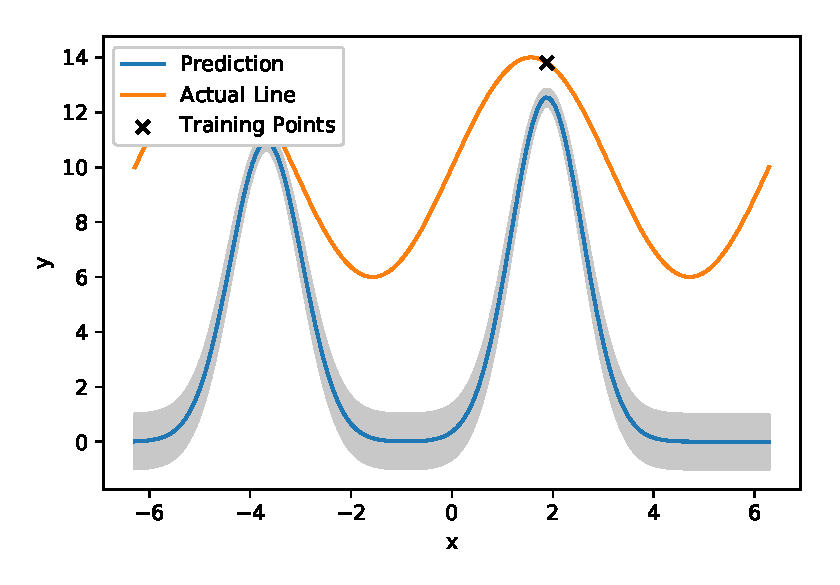
\includegraphics[width=\textwidth]{images/GP_Explanation/zero_const_mean_2_training.eps}
        
        \caption{Prior Belief: $y=0$. No of Training Points: 2}
        \label{fig:gp_plot_y0_2}
\end{minipage}%
\begin{minipage}{.5\textwidth}
  \centering
        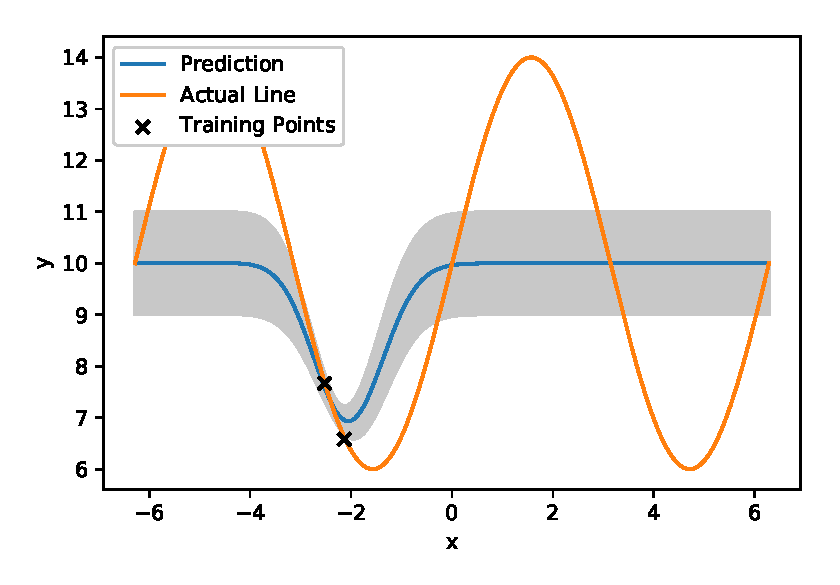
\includegraphics[width=\textwidth]{images/GP_Explanation/10_const_mean_2_training.eps}
        \caption{Prior Belief: $y=10$. No of Training Points: 2}
        \label{fig:gp_plot_y10_2}
\end{minipage}
\end{figure}


\begin{figure}[H]
\centering
\begin{minipage}{.5\textwidth}
  \centering
        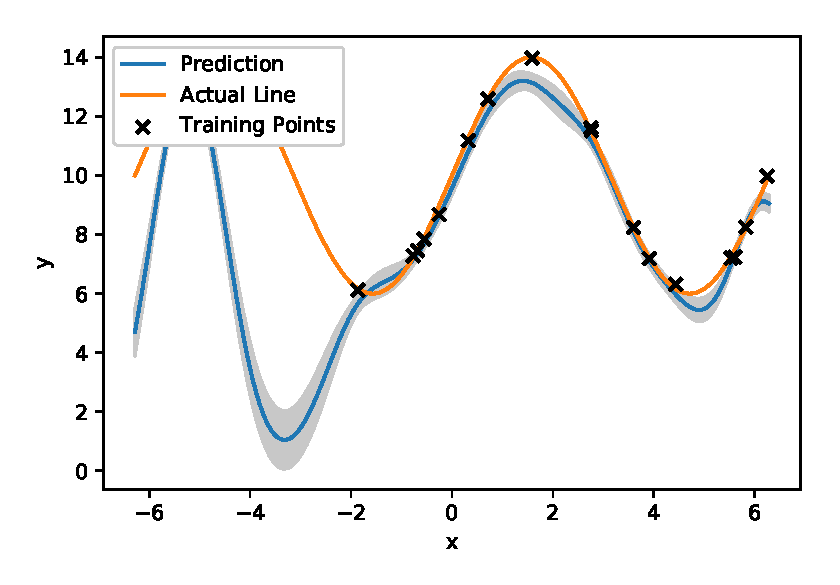
\includegraphics[width=\textwidth]{images/GP_Explanation/zero_const_mean_20_training.eps}
        
        \caption{Prior Belief: $y=0$. No of Training Points: 20}
        \label{fig:gp_plot_y0_20}
\end{minipage}%
\begin{minipage}{.5\textwidth}
  \centering
        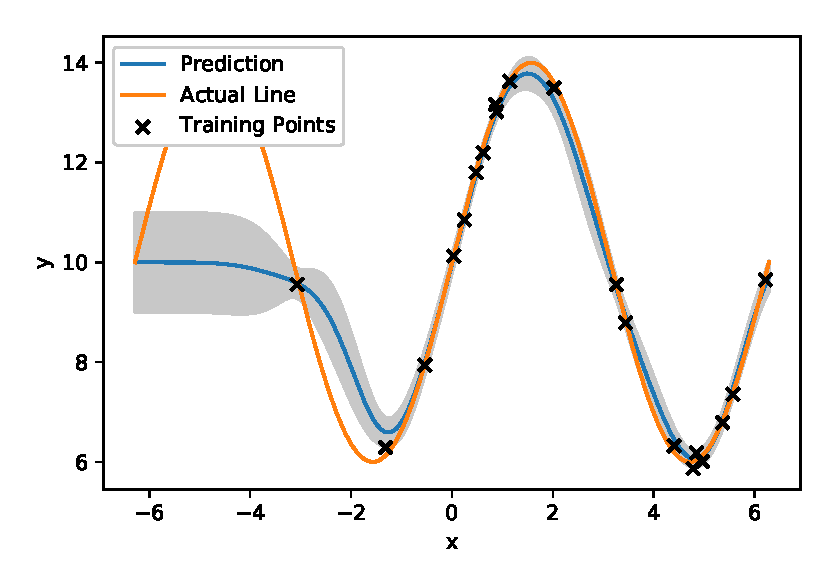
\includegraphics[width=\textwidth]{images/GP_Explanation/10_const_mean_20_training.eps}
        \caption{Prior Belief: $y=10$. No of Training Points: 20}
        \label{fig:gp_plot_y10_20}
\end{minipage}
\end{figure}




\begin{figure}[H]
\centering
\begin{minipage}{.5\textwidth}
  \centering
        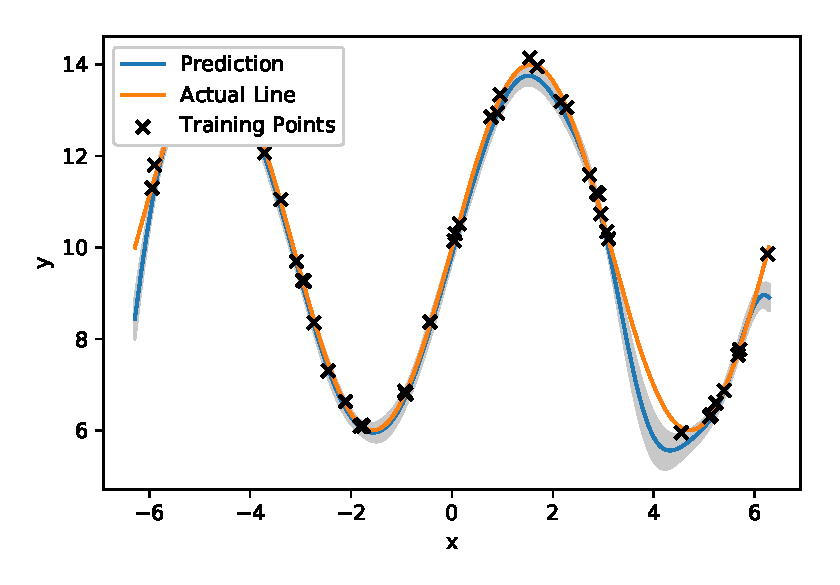
\includegraphics[width=\textwidth]{images/GP_Explanation/zero_const_mean_50_training.eps}
        
        \caption{Prior Belief: $y=0$. No of Training Points: 50}
        \label{fig:gp_plot_y0_50}
\end{minipage}%
\begin{minipage}{.5\textwidth}
  \centering
        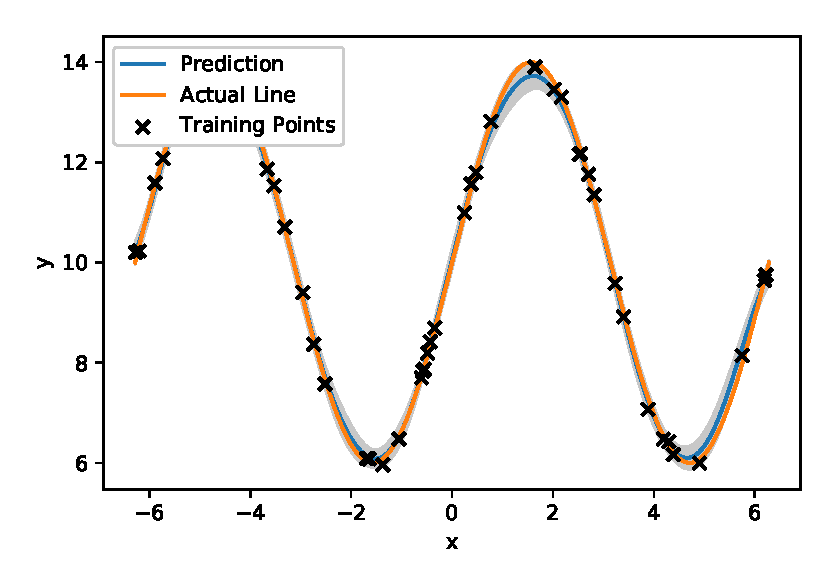
\includegraphics[width=\textwidth]{images/GP_Explanation/10_const_mean_50_training.eps}
        \caption{Prior Belief: $y=10$. No of Training Points: 50}
        \label{fig:gp_plot_y10_50}
\end{minipage}
\end{figure}



\begin{figure}[H]
\centering
\begin{minipage}{.5\textwidth}
  \centering
        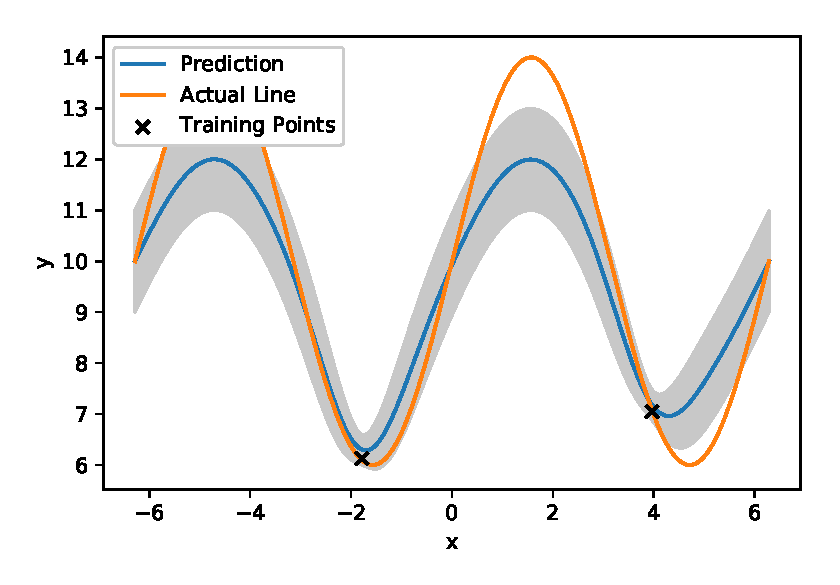
\includegraphics[width=\textwidth]{images/GP_Explanation/sin_mean_2_training.eps}
        
        \caption{Prior Belief: $y=2sin(x)+10$. No of Training Points: 2}
        \label{fig:gp_plot_y0_2}
\end{minipage}%
\begin{minipage}{.5\textwidth}
  \centering
        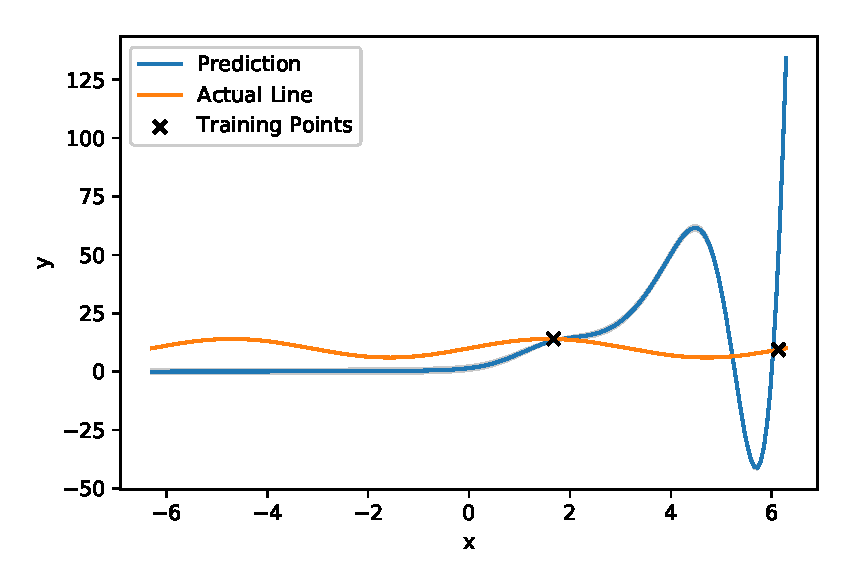
\includegraphics[width=\textwidth]{images/GP_Explanation/bad_mean_2_training.eps}
        \caption{Prior Belief: $y=e^x$. No of Training Points: 2}
        \label{fig:gp_plot_y10_2}
\end{minipage}
\end{figure}



\begin{figure}[H]
\centering
\begin{minipage}{.5\textwidth}
  \centering
        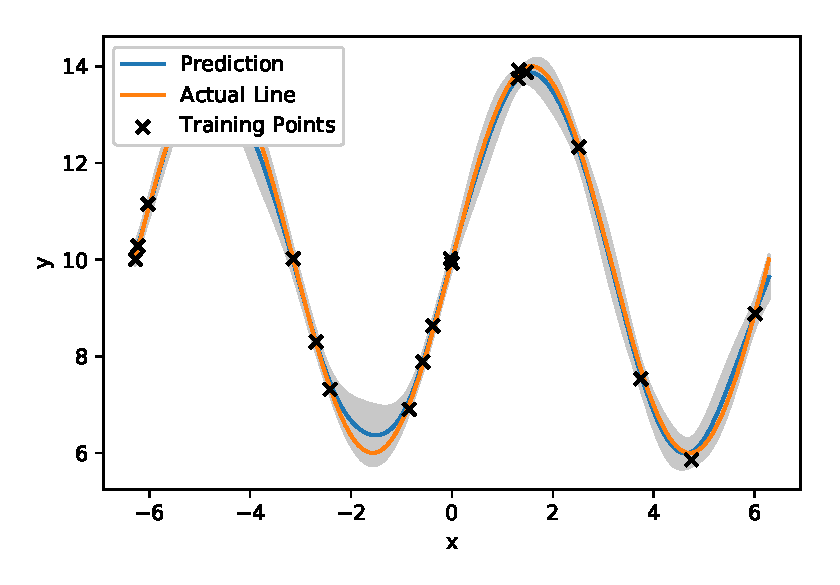
\includegraphics[width=\textwidth]{images/GP_Explanation/sin_mean_20_training.eps}
        
        \caption{Prior Belief: $y=2sin(x)+10$. No of Training Points: 20}
        \label{fig:gp_plot_y0_20}
\end{minipage}%
\begin{minipage}{.5\textwidth}
  \centering
        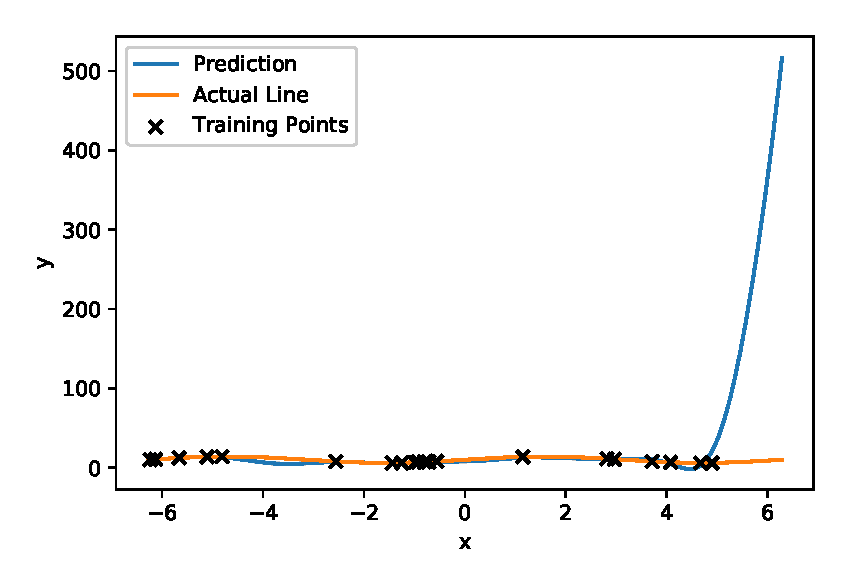
\includegraphics[width=\textwidth]{images/GP_Explanation/bad_mean_20_training.eps}
        \caption{Prior Belief: $y=e^x$. No of Training Points: 20}
        \label{fig:gp_plot_y10_20}
\end{minipage}
\end{figure}




\begin{figure}[H]
\centering
\begin{minipage}{.5\textwidth}
  \centering
        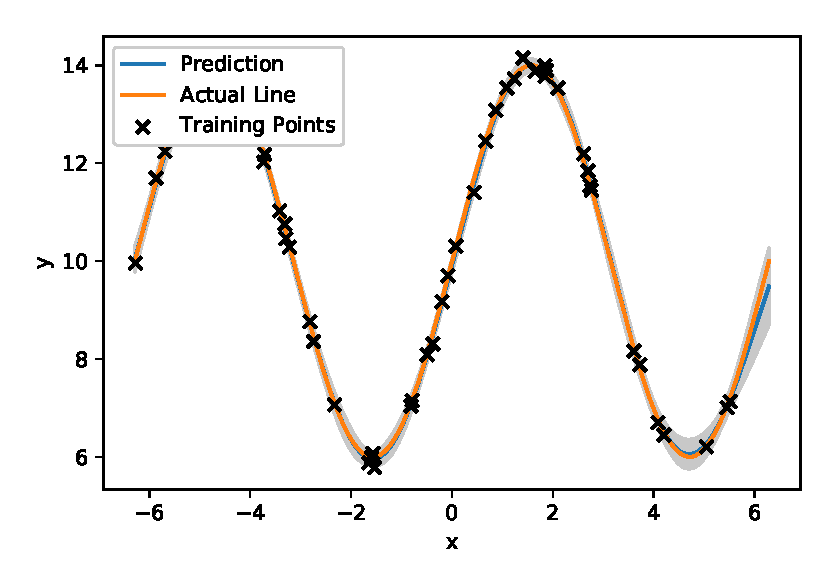
\includegraphics[width=\textwidth]{images/GP_Explanation/sin_mean_50_training.eps}
        
        \caption{Prior Belief: $y=2sin(x)+10$. No of Training Points: 50}
        \label{fig:gp_plot_y0_50}
\end{minipage}%
\begin{minipage}{.5\textwidth}
  \centering
        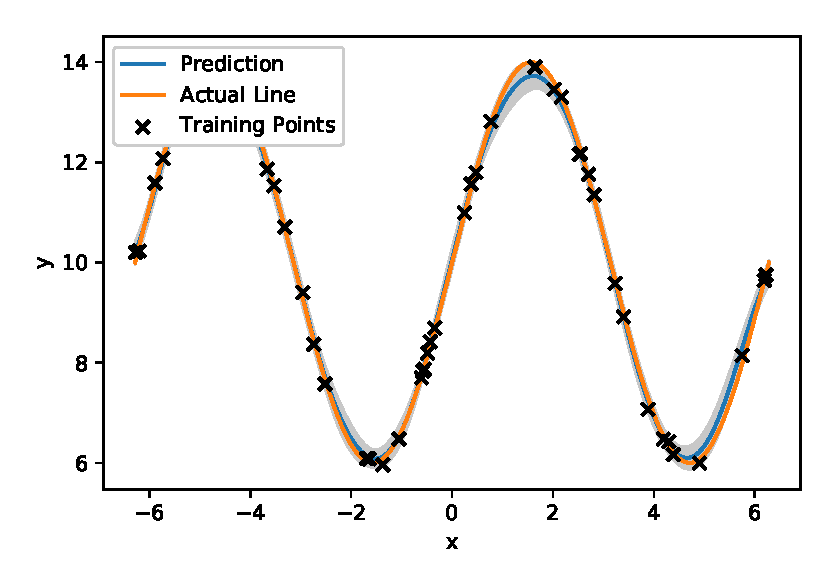
\includegraphics[width=\textwidth]{images/GP_Explanation/10_const_mean_50_training.eps}
        \caption{Prior Belief: $y=e^x$. No of Training Points: 50}
        \label{fig:gp_plot_y10_50}
\end{minipage}
\end{figure}



Confidence interval becomes largers for input values that are distant from any training points. 







\begin{figure}[H]
    \centering
    \includegraphics[width = \textwidth]{images/Non_zero_mean_converge.eps}
    \caption{Convergence rates for prior beliefs}
    \label{fig:GPconvergence_rates}
\end{figure}

\begin{figure}[H]
    \centering
    \includegraphics[width=\textwidth]{images/Bad_Non_zero_mean_converge_change.eps}
    \caption{Convergence rates for prior beliefs with poor representation of underlying function}
    \label{fig:GPbad_prior}
\end{figure}








\begin{figure}[H]
\centering
\begin{minipage}{.5\textwidth}
  \centering
        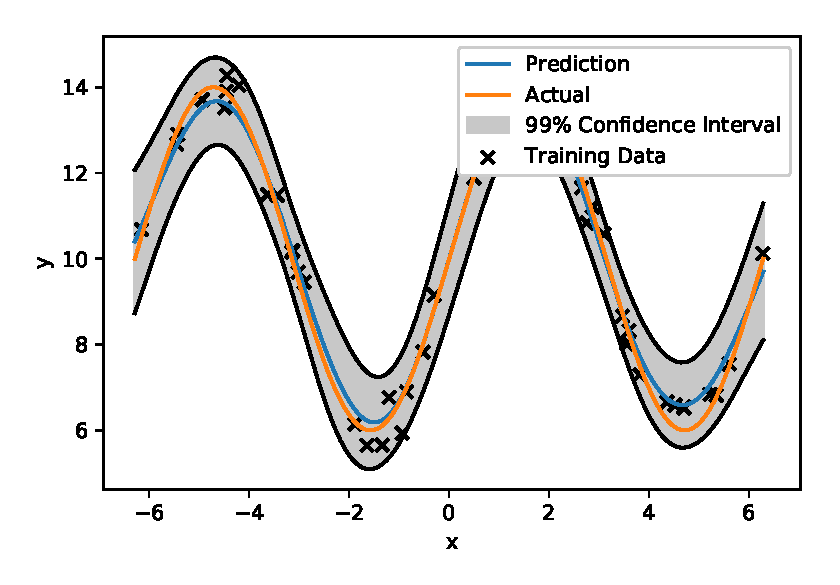
\includegraphics[width=\textwidth]{images/GP_Explanation/0_1_noise_confidence_interval.eps}
        
        \caption{Confidence Interval for a noisy sine wave $\epsilon = 0.1 $}
        \label{fig:0_1_confidence_interval}
\end{minipage}%
\begin{minipage}{.5\textwidth}
  \centering
        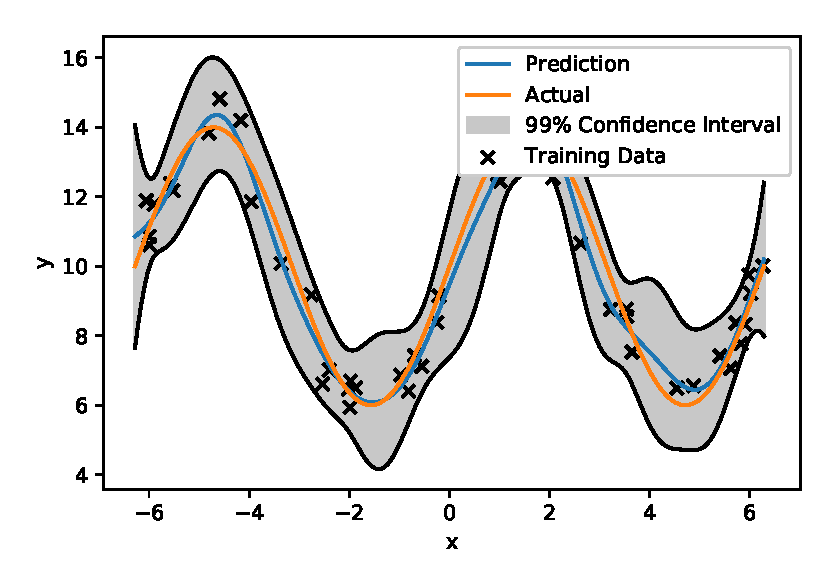
\includegraphics[width=\textwidth]{images/GP_Explanation/0_5_noise_confidence_interval.eps}
        \caption{Confidence Interval for a noisy sine wave $\epsilon = 0.5 $}
        \label{fig:0_5_confidence_interval}
\end{minipage}
\end{figure}